\begin{longtable} { | c | p{12cm} | c | } 
\hline
	ID 	&	Issues	&		 Es. hours \\\hline
	 47	&	Sequenceviewer: Dynamic show	&	16 hours \\\hline
\caption{Issue ID 47}
\label{tab:spr3_SVdynamicshow}
\end{longtable}

Sequenceviewer needed to be able to vary the number of pictograms to display. This issue originated from work done by the Requirements group during the semester, and can be seen in the requirement report in appendix \ref{app:reqgroup1}. The reason for this issue comes from the difference in the abilities that children possess. The different institutions who will work with this system, has children with varying strengths and weaknesses. Some children can only perform one task at a time, and should only have the next activity to look at. Some children however may be capable of seeing the entire sequence of activities at once. 

The varying number of pictograms to display, would be based on a setting provided by the application calling Sequenceviewer.

This issue was solved by first using one of two GComponents called GHorizontalScrollViewSnapper or GVerticalScrollViewSnapper. The collaboration with GComponents about creating these two components can be seen in section \ref{collaborationSnapper}. Horizontal is used for making landscape scrolling, and vertical for portrait. As both screen-orientations are built the same way, only landscape-mode is explained here. 

When Sequenceviewer is called, it launches \ct{onCreate} together with $\_$main.xml. In \ct{onCreate} a condition checks whether the calling application has requested landscape or portrait, see listing \ref{lst:landscapeDynamic}. In the case of landscape-mode, the layout in landscape$\_$mode.xml is inflated into activity$\_$main.xml. landscape$\_$mode.xml contains the GComponents regarding buttons, images and text for the Sequenceviewer. In \ct{onCreate} the colors from GComponents are set up using the \ct{setColors} method. Then the ScrollView for landscape-mode is created by instantiating a new \ct{HorizontallyScroll} view. \ct{HorizontallyScroll} takes 5 paremeters:
\begin{itemize}
\item \textit{Context context}, the current context.
\item \textit{Sequence sequence}, the sequence to display. This is gathered from the database by its id, sent from the calling application as \ct{intent}.
\item \textit{String type}, the name of the calling application.
\item \textit{View p}, the view in which the HorizontallyScroll view is added.
\item \textit{int picVisCount}, the number of visible pictograms. Sent by the calling application as \ct{intent}.
\end{itemize}

The ScrollView is then added to the relative layout in the landscape-layout.

\begin{lstlisting} [caption={Dynamic number of pictograms in landscape-mode}, label={lst:landscapeDynamic}]

setRequestedOrientation(ActivityInfo.SCREEN_ORIENTATION_LANDSCAPE);
View landscape = inflater.inflate(R.layout.landscape_mode, null);
mainView.addView(landscape);
	
setColors();
	
HorizontallyScroll horizontalScrolling = new HorizontallyScroll(this, sequence, type, landscape, numberOfVisibiblePictograms);
horizontalScrolling.setTag("land_hscrollview");
horizontalScrolling.setLayoutParams(new HorizontalScrollView.LayoutParams(HorizontalScrollView.LayoutParams.MATCH_PARENT, HorizontalScrollView.LayoutParams.MATCH_PARENT));
RelativeLayout land_rellay = (RelativeLayout) landscape.findViewById(R.id.landscape_rellay);
land_rellay.addView(horizontalScrolling);
\end{lstlisting}

By Android defined standards, multiple views cannot be directly added to a \ct{ScrollView}. Therefore, in the constructor of \ct{HorizontallyScroll}, a \ct{LinearLayout} is created and added to the \ct{ScrollView} called \ct{mainLayout}. 

Next thing was to create a view in the \ct{ScrollView} for each pictogram in the sequence. This was done by first overriding \ct{onDraw} in \ct{HorizontallyScroll}. We need to work with the width and height of the view in which the \ct{ScrollView} exists, and Android does not define width and height before it has drawn the view. For each pictogram, we instantiated a new \ct{PictogramView}. Before we added the pictogram to the view, we had to consider the number of pictograms to display. Therefore we scale it. We define the limiting factor in the view by using $math.min$, which returns the most negative of two argument. We feed $math.min$ with \ct{getWidth() / numberOfVisibiblePictograms} and \ct{getHeight}. As this is landscape-mode, they line up horizontally. Therefore we divide the width into a section for each requested visible pictogram. Then a pictogramScaling-method is called, refer listing \ref{lst:pictogramScalingMethod}, which makes the pictograms as large as possible, within the section they are allowed fill. The method takes the original pictogram, the limiting factor and a filter. We do however not use filters. If the pictogram is larger than 100 in width or height, it is scaled down to around 100x100. Thereafter, it scales the pictogram up or down to match the assigned section. 

\begin{lstlisting} [caption={Scaling method for pictograms}, label={lst:pictogramScalingMethod}]

protected Bitmap pictogramScaling(Bitmap realImage, float maxImageSize, boolean filter){

    if(realImage.getWidth() > 100 || realImage.getHeight() > 100) {
        float ratio = Math.max((float) realImage.getWidth() / 100, (float) realImage.getHeight() / 100);
        realImage = Bitmap.createScaledBitmap(realImage, Math.round((float) realImage.getWidth() / ratio),  Math.round((float) realImage.getHeight() / ratio), filter);
    }

    float ratio = Math.min((float) maxImageSize / realImage.getWidth(), (float) maxImageSize / realImage.getHeight());

    int width = Math.round((float) ratio * realImage.getWidth());
    int height = Math.round((float) ratio * realImage.getHeight());

    Bitmap newBitmap = Bitmap.createScaledBitmap(realImage, width, height, filter);
    newBitmap.setDensity(0);
    return newBitmap;
}
\end{lstlisting}

At this point, the pictogram is added to the \ct{PictogramView}. \ct{PictogramView} is a class taken from the Sekvens, which creates rounded edges on the pictogram. Then, the \ct{PictogramView} is added to the before mentioned \ct{LinearLayout} called \ct{mainLayout}, which contains all the pictograms to display.

The last thing we do is to scale the layout-parameters of the \ct{ScrollView} and \ct{mainLayout}. We define the width as: \ct{pictogramToDisplay.getWidth()* numberOfVisibiblePictograms}, and define the height as: \ct{RelativeLayout.LayoutParams.MATCH$\_$PARENT}. The \ct{pictogramToDisplay} is a regular pictogram that is scaled the same way as those in a sequence, which we use to get a pictogram width. We define these layout-parameters for the \ct{ScrollView} and the \ct{mainLayout}, and then center everything in the \ct{mainLayout} by calling \ct{mainLayout.setGravity(Gravity.CENTER)}, refer listing \ref{lst:addPictogram}.

\begin{lstlisting} [caption={Adding the scaled pictogram to the PictogramView}, label={lst:addPictogram}]
limiter = Math.min(getWidth() / numberOfVisibiblePictograms, getHeight());
Bitmap pictogramToDisplay = pictogramScaling(pictogram, limiter, false);
pictoView.setImageFromBitmap(pictogramToDisplay);
	mainLayout.addView(pictoView);
\end{lstlisting}

The \ct{VerticallyScroll} is made the same way, but here it is the height which is divided into section. In figure \ref{fig:portrait3pics} and \ref{fig:portrait5pics}, portrait-mode is displayed with two different settings. It scales the pictograms accordingly, and limits the \ct{ScrollView} when the pictograms are not filling the entire height.

\begin{figure}[ht!]
\centering
\begin{minipage}{.45\textwidth}
\centering
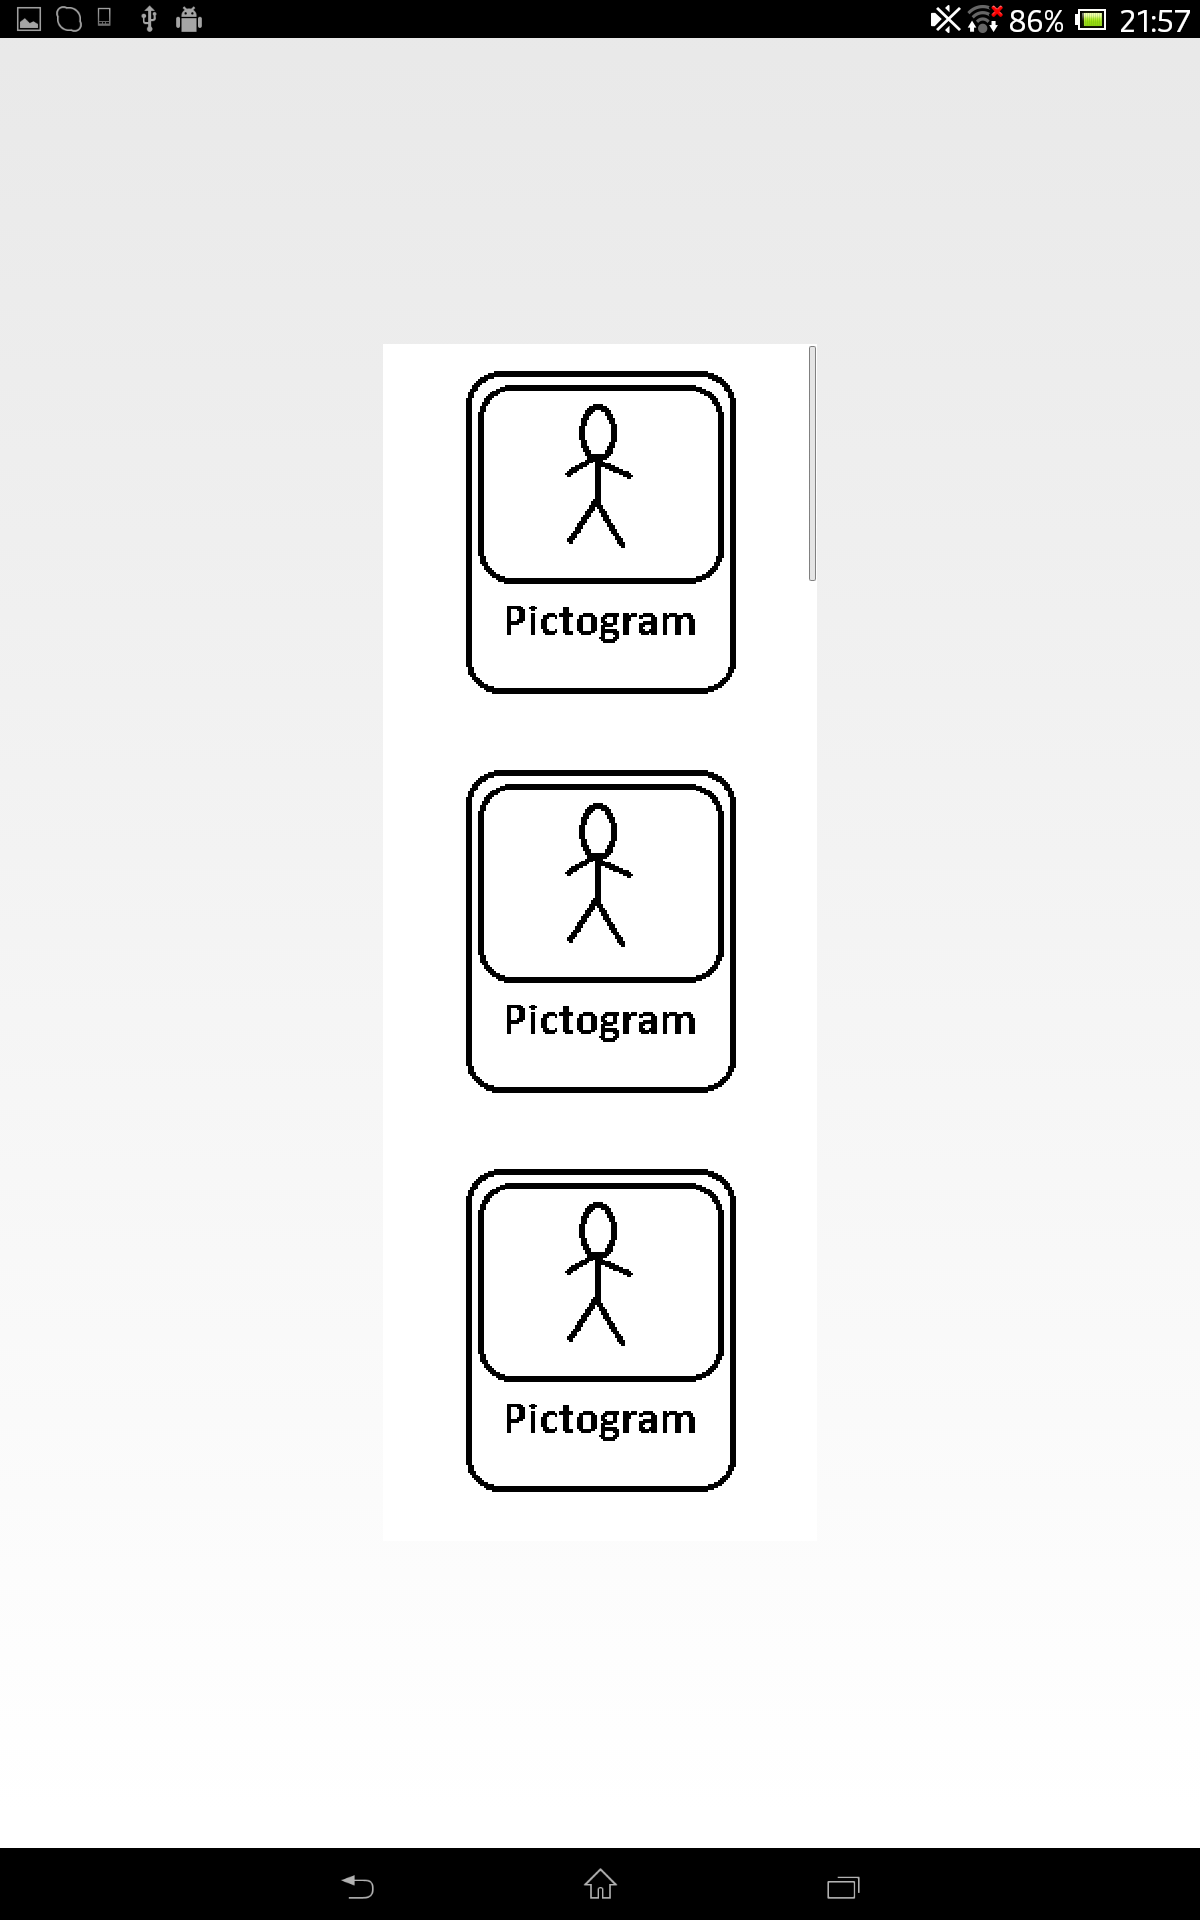
\includegraphics[scale=0.1]{Pics/Sprint3/portrait3pics.png}
\caption{A sequence displayed with 3 visible pictograms in portrait-mode}
\label{fig:portrait3pics}
\end{minipage}\hfill
\begin{minipage}{.45\textwidth}
\centering
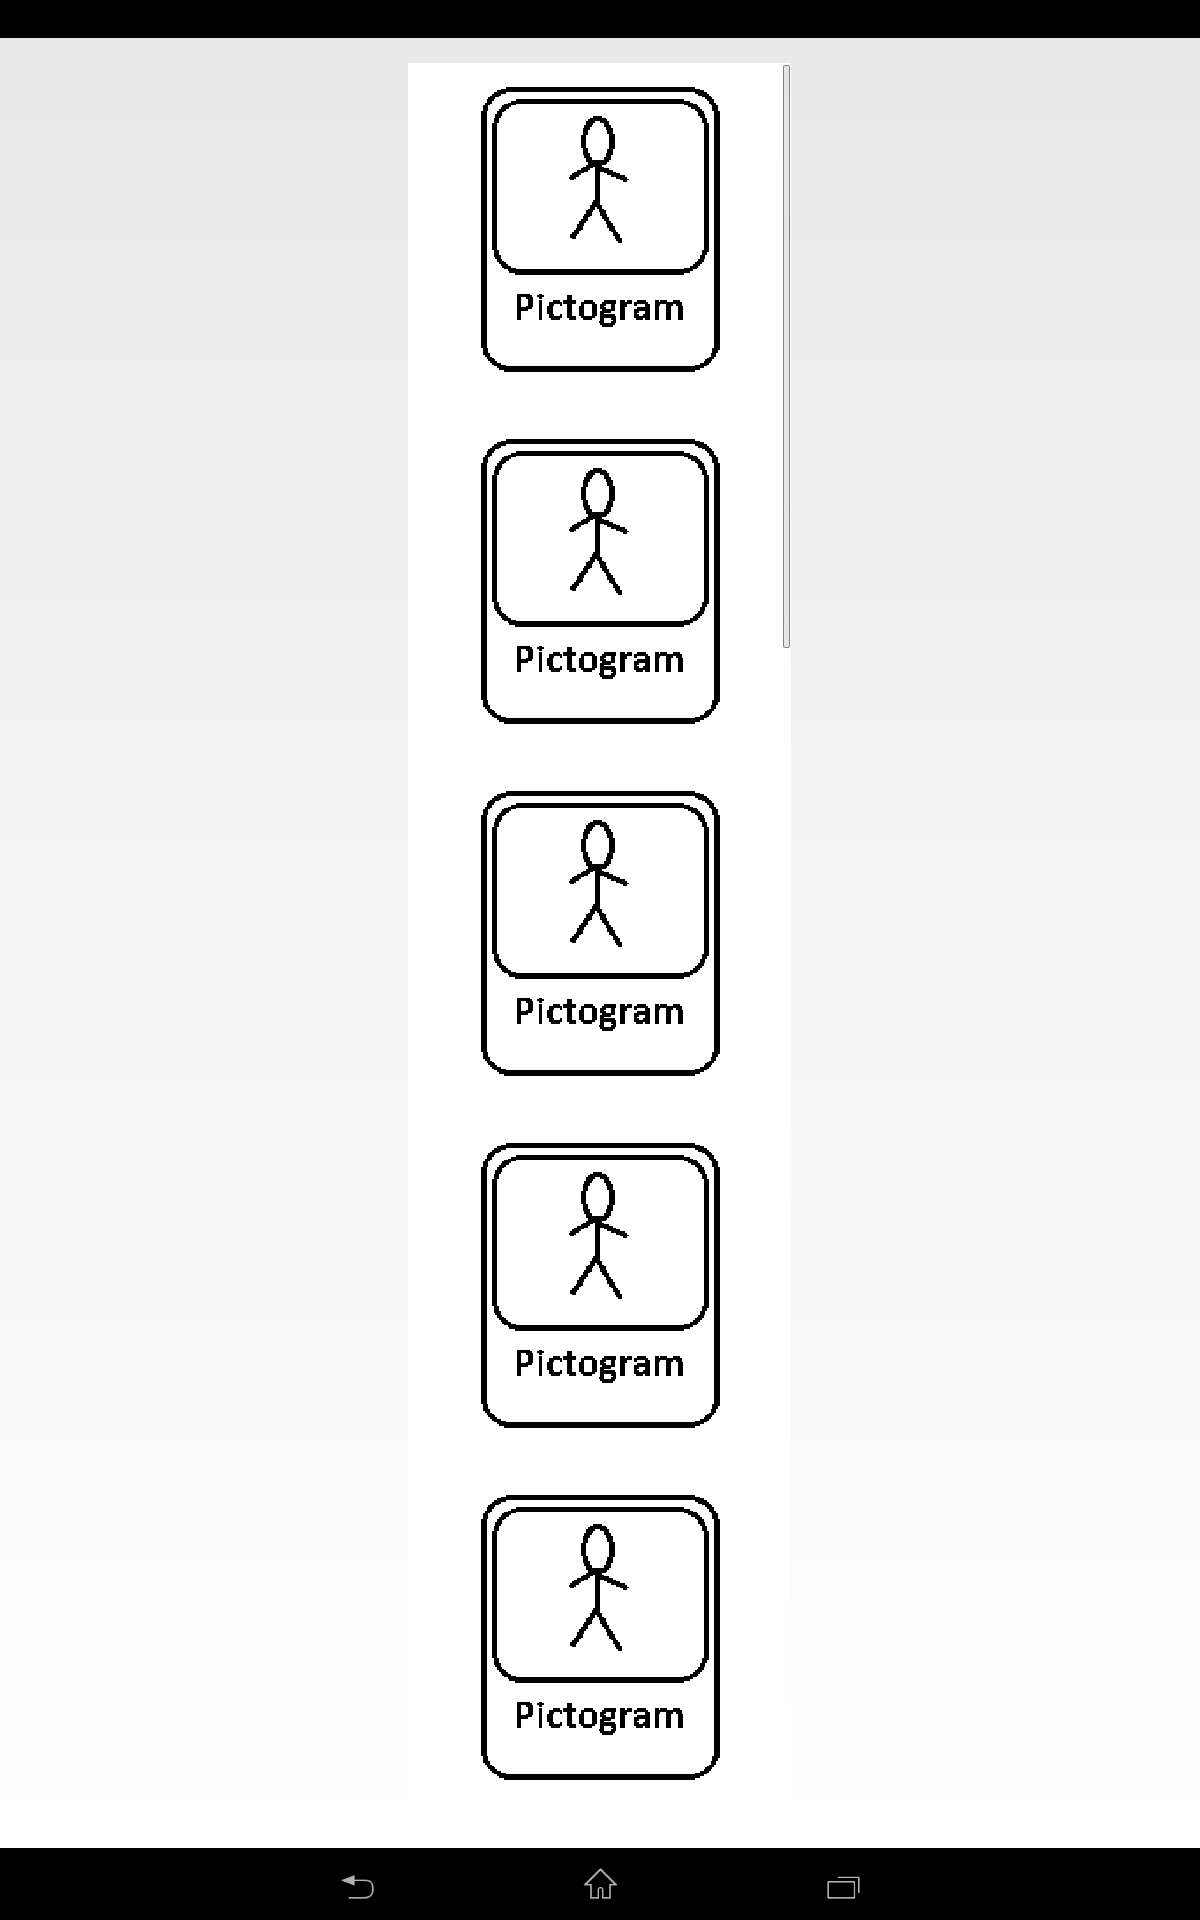
\includegraphics[scale=0.1]{Pics/Sprint3/portrait5pics.png}
\caption{A sequence displayed with 5 visible pictograms in portrait-mode}
\label{fig:portrait5pics}
\end{minipage}
\end{figure}















